% BCSP States of Consciousness 2026 poster. 48 x 36 inches, horizontal.
% Build: tectonic poster.tex   Print at 100 percent scale, no fit-to-page.
% Before printing in October: add the paper 1 DOI QR next to the repo QR
% (slot reserved in the title band) once PsyArXiv moderation clears.
\documentclass[11pt]{article}
\usepackage[paperwidth=48in,paperheight=36in,margin=0in]{geometry}
\usepackage{lmodern}
\usepackage[T1]{fontenc}
\usepackage{graphicx}
\graphicspath{{../}{.}}
\usepackage{xcolor}
\usepackage[absolute,overlay]{textpos}
\usepackage{tcolorbox}
\usepackage{enumitem}
\setlength{\TPHorizModule}{1in}
\setlength{\TPVertModule}{1in}
\setlength{\parindent}{0pt}
\pagestyle{empty}
\renewcommand{\familydefault}{\sfdefault}

\definecolor{slate}{HTML}{1F2A36}
\definecolor{accent}{HTML}{B2182B}
\definecolor{panelbg}{HTML}{F7F8FA}
\definecolor{rule}{HTML}{D5DAE0}

\tcbset{poster/.style={colback=panelbg, colframe=rule, boxrule=1.2pt, arc=4mm,
  left=0.28in, right=0.28in, top=0.22in, bottom=0.22in}}

\newcommand{\panelhead}[1]{{\fontsize{40}{46}\selectfont\bfseries\color{slate}#1}\\[0.14in]
{\color{accent}\rule{2.6in}{3pt}}\\[0.2in]}
\newcommand{\body}[1]{{\fontsize{24}{31}\selectfont\color{slate}#1}}
\newcommand{\pcap}[1]{{\fontsize{21}{27}\selectfont\color{slate}#1}}

\begin{document}
\null

% ---------------- title band ----------------
\begin{textblock*}{40in}(0.7in,0.55in)
{\fontsize{96}{100}\selectfont\bfseries\color{slate}What the Theory Never Specifies\par}
\vspace{0.18in}
{\fontsize{46}{52}\selectfont\color{accent}\bfseries Preregistered Simulations of REBUS and ALBUS\par}
\vspace{0.22in}
{\fontsize{32}{38}\selectfont\color{slate}Joshua Rogers\quad\textperiodcentered\quad
independent researcher\quad\textperiodcentered\quad josh@envitae.io\par}
\end{textblock*}

\begin{textblock*}{6.0in}(41.2in,0.5in)
\begin{center}

\includegraphics[width=2.35in]{qr_repo.png}\\[0.05in]
{\fontsize{17}{21}\selectfont\color{slate}\bfseries code, preregistrations, results, both papers\\
github.com/ArtHangup/rebus-albus-sim\par}
\end{center}
\end{textblock*}

% ---------------- row 1 ----------------
\begin{textblock*}{13.6in}(0.7in,4.15in)
\begin{tcolorbox}[poster, height=10.05in]
\panelhead{The question, the agent, the rules}
\body{Why do some psychedelic sessions produce lasting change while others change
nothing, or leave a person more convinced of the belief that harms them? REBUS says
the drug relaxes rigid priors so beliefs can revise. ALBUS says low doses strengthen
them. Neither theory has ever been implemented.\\[0.22in]
\textbf{The agent} is the minimal Bayesian belief-updater both theories describe:
six hypotheses, one true, one a maladaptive conviction held at 3000 to 1 odds, and a
dose that does exactly one thing, relax the prior's weight while evidence arrives:
$\gamma(d)=\gamma_0(1-d)$.\\[0.22in]
\textbf{The rules:} every mapping was committed to a public git history before the
code that tested it existed, across 11 amendments and 44 numbered predictions.
Predictions that failed are reported on this poster, because the failures produced
the best results.}
\end{tcolorbox}
\end{textblock*}

\begin{textblock*}{32.35in}(14.75in,4.15in)
\begin{tcolorbox}[poster, height=10.05in]
\panelhead{Nothing lasts as stated, and an unstated assumption decides whether the drug matters}
\begin{minipage}[t]{21.9in}
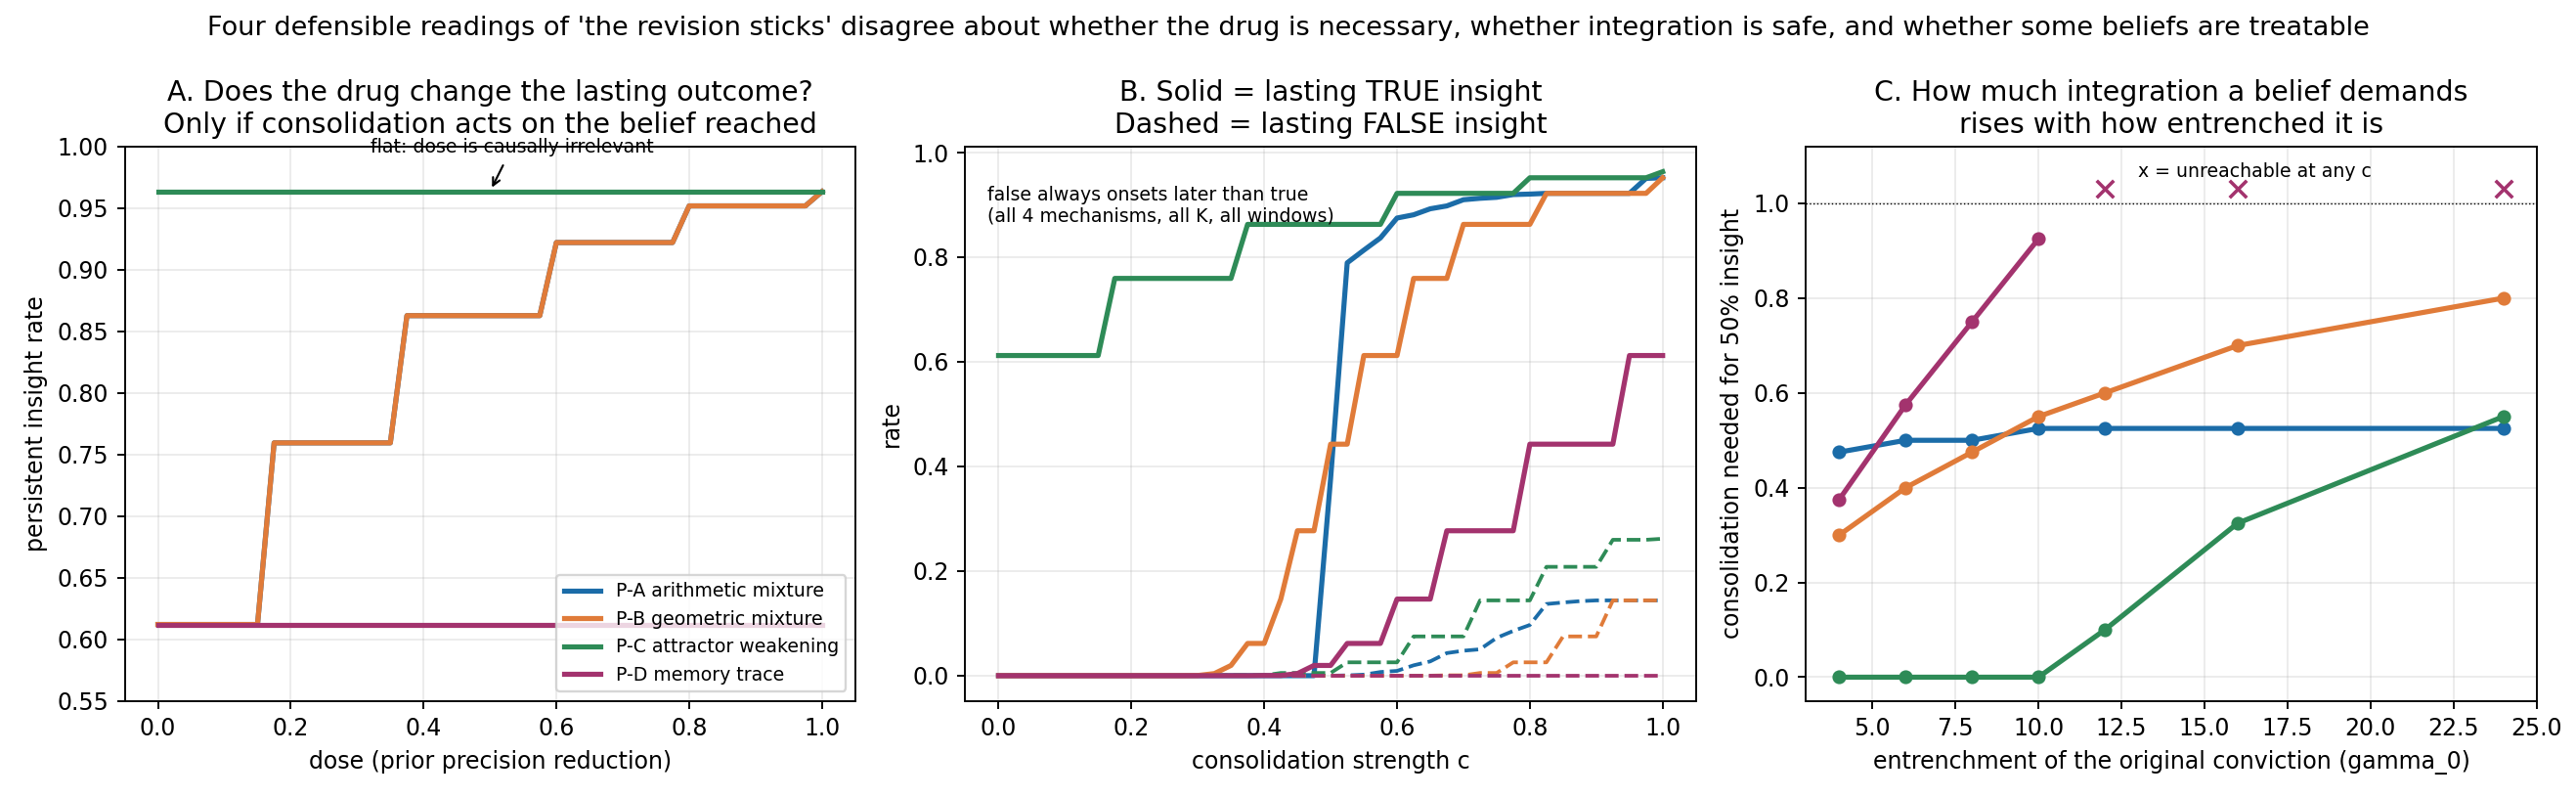
\includegraphics[width=21.9in]{figure_robustness.png}
\end{minipage}\hfill
\begin{minipage}[t]{8.9in}
\pcap{Literal REBUS produces zero lasting change: dose enters only through a precision
that reverts, so it cannot reach the outcome. Consolidation must be added, and it acts
as a gate. But four defensible readings of what consolidation operates on disagree
about whether the drug matters at all (under the attractor reading, dose zero is
best), whether integration can be made safe, and whether entrenched beliefs are
treatable. Neither REBUS nor REBAS states which reading is right; each is measurable.}
\end{minipage}
\end{tcolorbox}
\end{textblock*}

% ---------------- row 2 ----------------
\begin{textblock*}{15.1in}(0.7in,14.5in)
\begin{tcolorbox}[poster, height=10.0in]
\panelhead{Strengthening is avoidance}
\begin{center}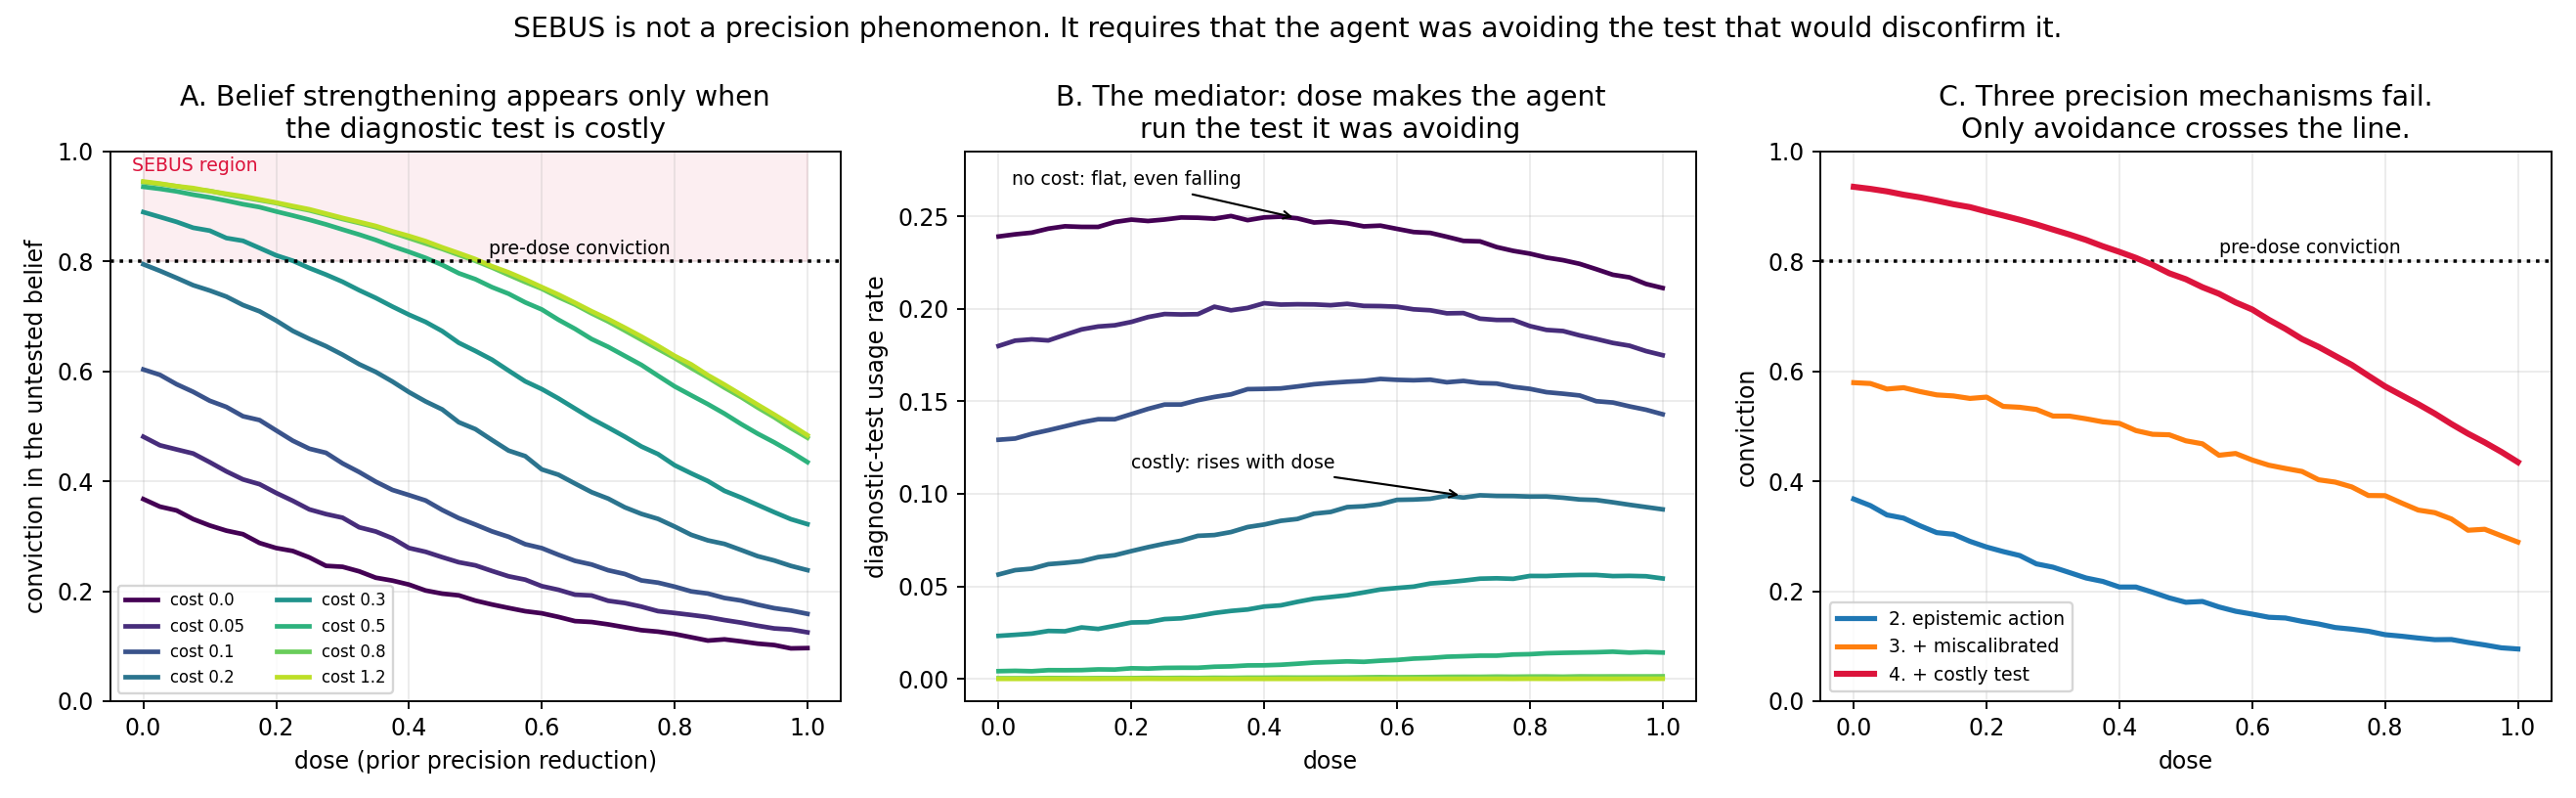
\includegraphics[width=14.3in]{figure_acting.png}\end{center}
\pcap{SEBUS never emerges from precision mechanics: passive relaxation, epistemic
action, and miscalibrated self-knowledge all fail. It appears only when the one
diagnostic test carries a cost the agent declines to pay. The mediator shows the
drug's derivable role: relaxation raises the value of the avoided test until it is
worth running. Above a cost ceiling, no dose helps.}
\end{tcolorbox}
\end{textblock*}

\begin{textblock*}{15.1in}(16.35in,14.5in)
\begin{tcolorbox}[poster, height=10.0in]
\panelhead{ALBUS's own mechanism needs avoidance too}
\begin{center}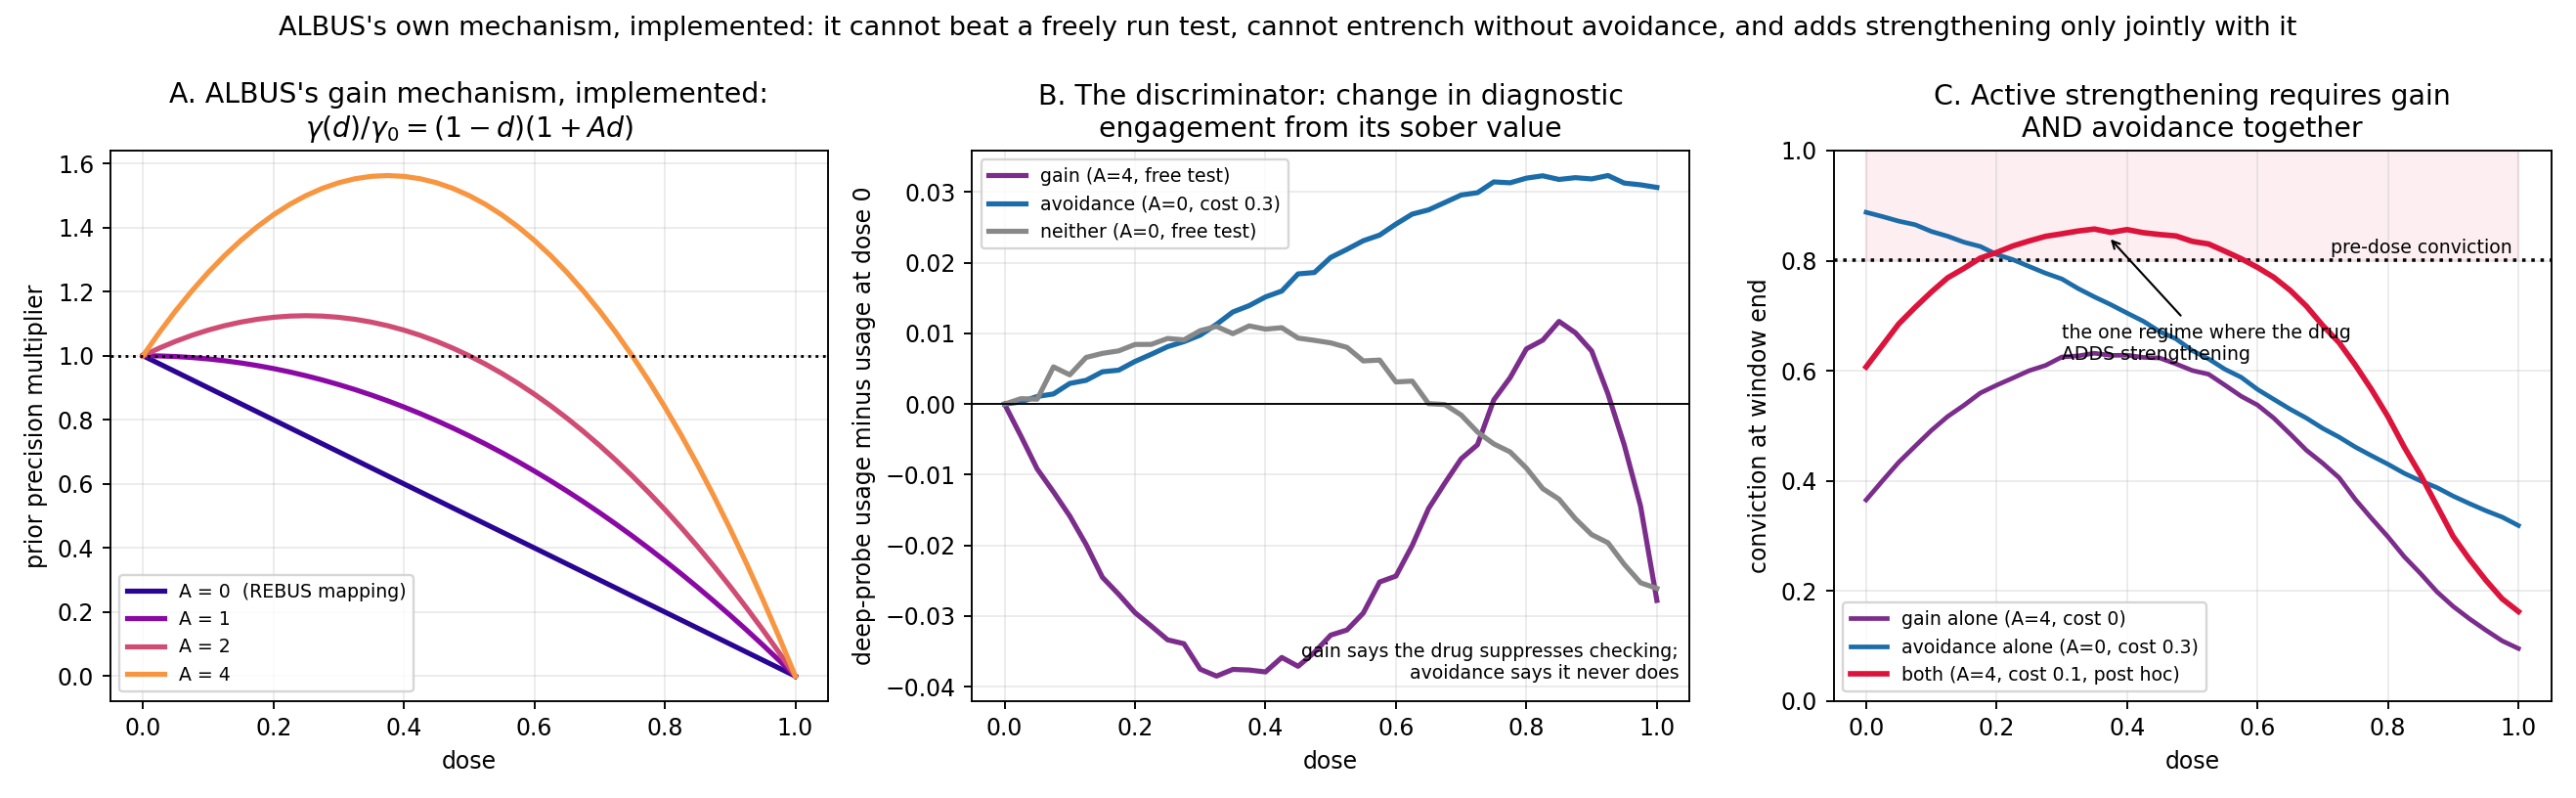
\includegraphics[width=14.3in]{figure_gain.png}\end{center}
\pcap{A low-dose gain increase, implemented honestly, cannot beat a freely run test
and cannot entrench without a cost. The accounts separate by sign: gain says the
drug suppresses checking at low dose, avoidance says it never does. Drug-added
strengthening exists in one confirmed regime only: gain and cost together.}
\end{tcolorbox}
\end{textblock*}

\begin{textblock*}{15.1in}(32.0in,14.5in)
\begin{tcolorbox}[poster, height=10.0in]
\panelhead{The therapeutic window is three-dimensional}
\begin{center}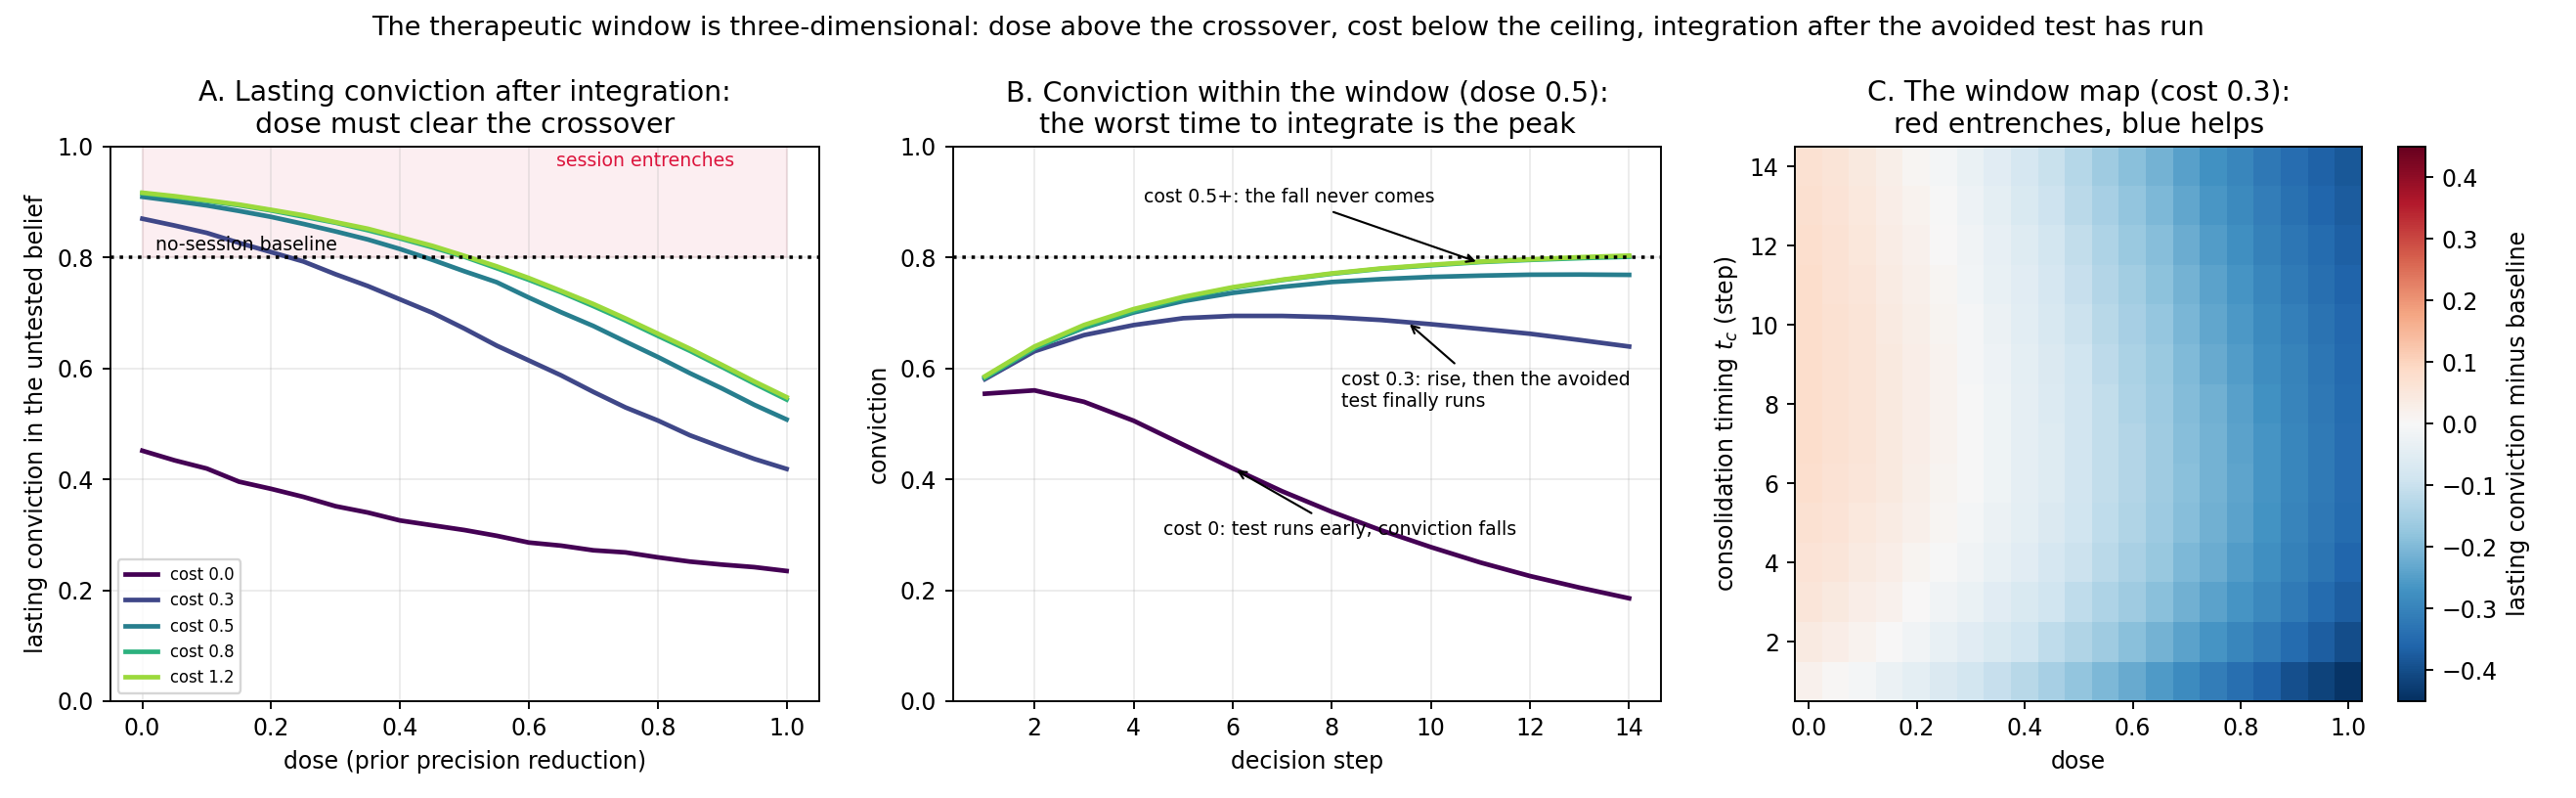
\includegraphics[width=14.3in]{figure_window.png}\end{center}
\pcap{Dose must clear a cost-dependent crossover, cost must sit below the ceiling,
and integration must capture the state after the avoided test has run. Miss a
coordinate and the same session entrenches the belief, or dissolves it without
replacing it: lasting conviction falls while insight never arrives.}
\end{tcolorbox}
\end{textblock*}

% ---------------- row 3 ----------------
\begin{textblock*}{29.6in}(0.7in,24.85in)
\begin{tcolorbox}[poster, height=10.45in, colframe=accent, boxrule=2.4pt]
\panelhead{The ratchet: how a belief becomes chronic}
\begin{center}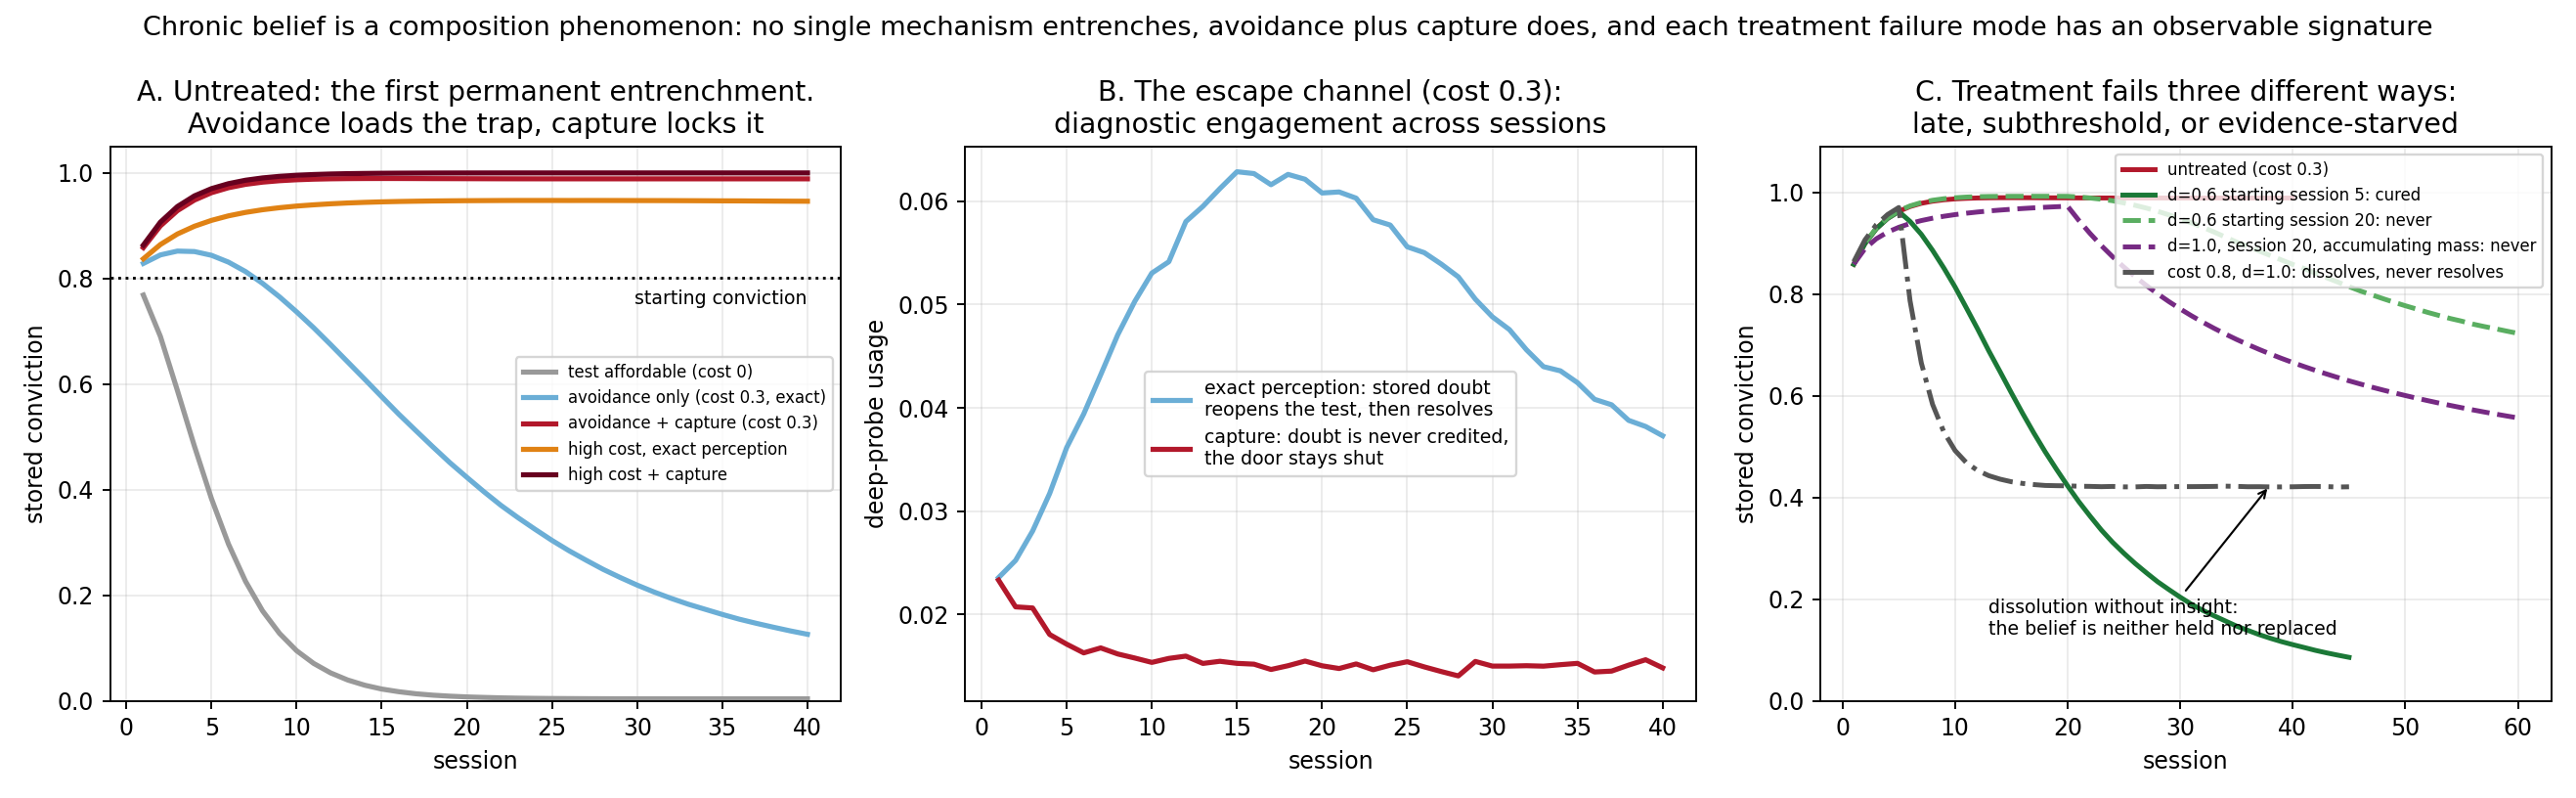
\includegraphics[width=24.9in]{figure_ratchet.png}\end{center}
\pcap{Avoidance alone is self-limiting: refusing the test stores up the doubt that
eventually reopens it. Biased interpretation never credits that doubt: conviction
climbs from 0.80 to 0.99 and locks. \textbf{Avoidance loads the trap, capture locks
it.} Treatment fails three observable ways: the dose never opens the test, the belief
dissolves without being replaced, or memory outruns the course.}
\end{tcolorbox}
\end{textblock*}

\begin{textblock*}{16.25in}(30.85in,24.85in)
\begin{tcolorbox}[poster, height=10.45in]
\panelhead{What to take home}
\body{\begin{itemize}[leftmargin=0.55in, itemsep=0.16in]
\item Integration, not dose, gates lasting change; which quantity it operates on is
an unstated assumption that flips the answer.
\item The drug's derivable role is to make an avoided disconfirming test worth
running: the exposure account of therapy, emerging from REBUS's own vocabulary.
\item Rigid beliefs defend themselves through what you do (avoidance), what you see
(capture), and what counts (gain); only compositions entrench.
\item One behavioral marker separates every account: engagement with avoided
disconfirming evidence, by sign and by trajectory.
\end{itemize}
\vspace{0.12in}\par
Belief dynamics only: no claim about phenomenal experience. The same
implement-and-see discipline on machine implementations of global workspace theory
gave the same lesson: the unstated assumptions decide.}
\end{tcolorbox}
\end{textblock*}

\end{document}
